% =====================================================================
% fig:layerlaw (IEEE de-merge, part 1 of former figA_lawtransfer / F1+F7).
% Layer-law panels only: (a) depth, (b) regime-across-scale. The
% architecture-generalization panels move to the companion single-column
% figure fig:crossarch (figA2_crossarch.tex), referenced from
% Section~\ref{sec:dissociation}.
% Body ported from the R/tikzDevice pipeline (figures/figA1.tex, IEEE
% dimensions) rather than hand-authored pgfplots, for consistency with the
% rest of the figure set. Same source JSONs, no new numbers.
% Regenerate: Rscript figures/make_figures_ieee.R
% =====================================================================
\begin{figure*}[t]
\centering
% =====================================================================
% figA1  — R/ggplot2 -> tikzDevice (parallel to ../figures-tex/figA1_layerlaw.tex)
% Canonical-JSON-only. Regenerate: Rscript figures/make_figures_ieee.R
% Provenance (JSON path :: field = plotted value), one line per series:
% SOURCE: results/G1_L8_analysis.json :: aggregate.within_probe_mean_across_seeds = 0.3951
% SOURCE: results/G1_L8_analysis.json :: mean(per_seed[].within_probe_mean_normgrowth) = 0.0825
% SOURCE: results/G1_L10_analysis.json :: aggregate.within_probe_mean_across_seeds = 0.5337
% SOURCE: results/G1_L10_analysis.json :: mean(per_seed[].within_probe_mean_normgrowth) = 0.2458
% SOURCE: results/G1_L12_analysis.json :: aggregate.within_probe_mean_across_seeds = 0.6018
% SOURCE: results/G1_L12_analysis.json :: mean(per_seed[].within_probe_mean_normgrowth) = 0.5087
% SOURCE: results/G1_L14_analysis.json :: aggregate.within_probe_mean_across_seeds = 0.3006
% SOURCE: results/G1_L14_analysis.json :: mean(per_seed[].within_probe_mean_normgrowth) = 0.5019
% SOURCE: results/C3_regime_3b_L24_r4.json :: aggregate.within_probe_mean_across_seeds = 0.3764
% SOURCE: results/C3_llama8b_r3.json :: per_seed[L16].within_probe_mean = 0.1734
% SOURCE: results/C3_llama8b_r3.json :: per_seed[L24].within_probe_mean = -0.1169
% SOURCE: results/C3_llama8b_r3.json :: per_seed[L28].within_probe_mean = 0.1554
% =====================================================================
% !TEX encoding = UTF-8 Unicode
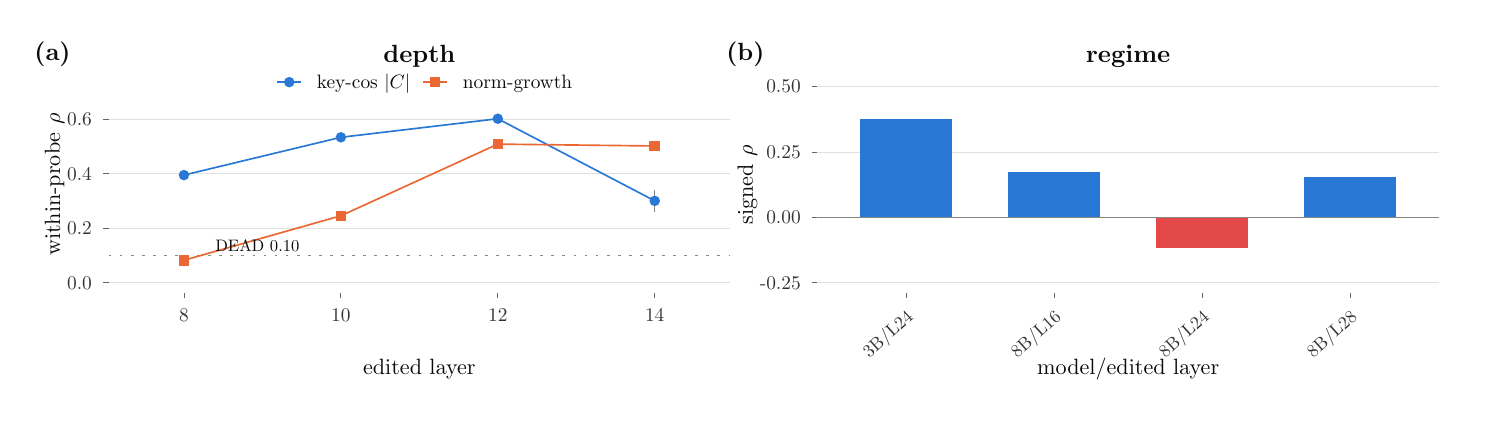
\begin{tikzpicture}[x=1pt,y=1pt]
\definecolor{fillColor}{RGB}{255,255,255}
\path[use as bounding box,fill=fillColor,fill opacity=0.00] (0,0) rectangle (517.45,133.70);
\begin{scope}
\path[clip] (  0.00,  0.00) rectangle (517.45,133.70);
\definecolor{drawColor}{RGB}{255,255,255}
\definecolor{fillColor}{RGB}{255,255,255}

\path[draw=drawColor,line width= 0.6pt,line join=round,line cap=round,fill=fillColor] ( -0.00,  0.00) rectangle (517.45,133.70);
\end{scope}
\begin{scope}
\path[clip] (  5.50,  5.50) rectangle (255.81,128.20);
\definecolor{fillColor}{RGB}{255,255,255}

\path[fill=fillColor] (  5.50,  5.50) rectangle (255.81,128.20);
\end{scope}
\begin{scope}
\path[clip] (255.81,  5.50) rectangle (511.95,128.20);
\definecolor{fillColor}{RGB}{255,255,255}

\path[fill=fillColor] (255.81,  5.50) rectangle (511.95,128.20);
\end{scope}
\begin{scope}
\path[clip] ( 29.24, 37.97) rectangle (253.81,115.98);
\definecolor{drawColor}{RGB}{225,224,217}

\path[draw=drawColor,line width= 0.3pt,line join=round] ( 29.24, 41.52) --
	(253.81, 41.52);

\path[draw=drawColor,line width= 0.3pt,line join=round] ( 29.24, 61.22) --
	(253.81, 61.22);

\path[draw=drawColor,line width= 0.3pt,line join=round] ( 29.24, 80.91) --
	(253.81, 80.91);

\path[draw=drawColor,line width= 0.3pt,line join=round] ( 29.24,100.61) --
	(253.81,100.61);
\definecolor{drawColor}{RGB}{137,135,129}

\path[draw=drawColor,line width= 0.3pt,dash pattern=on 1pt off 3pt ,line join=round] ( 29.24, 51.37) -- (253.81, 51.37);

\path[draw=drawColor,line width= 0.4pt,line join=round] ( 56.46, 81.48) --
	( 56.46, 81.48);

\path[draw=drawColor,line width= 0.4pt,line join=round] ( 56.46, 81.48) --
	( 56.46, 79.39);

\path[draw=drawColor,line width= 0.4pt,line join=round] ( 56.46, 79.39) --
	( 56.46, 79.39);

\path[draw=drawColor,line width= 0.4pt,line join=round] (113.17, 95.12) --
	(113.17, 95.12);

\path[draw=drawColor,line width= 0.4pt,line join=round] (113.17, 95.12) --
	(113.17, 93.05);

\path[draw=drawColor,line width= 0.4pt,line join=round] (113.17, 93.05) --
	(113.17, 93.05);

\path[draw=drawColor,line width= 0.4pt,line join=round] (169.88,102.65) --
	(169.88,102.65);

\path[draw=drawColor,line width= 0.4pt,line join=round] (169.88,102.65) --
	(169.88, 98.93);

\path[draw=drawColor,line width= 0.4pt,line join=round] (169.88, 98.93) --
	(169.88, 98.93);

\path[draw=drawColor,line width= 0.4pt,line join=round] (226.59, 75.09) --
	(226.59, 75.09);

\path[draw=drawColor,line width= 0.4pt,line join=round] (226.59, 75.09) --
	(226.59, 67.15);

\path[draw=drawColor,line width= 0.4pt,line join=round] (226.59, 67.15) --
	(226.59, 67.15);
\definecolor{drawColor}{RGB}{42,120,214}

\path[draw=drawColor,line width= 0.6pt,line join=round] ( 56.46, 80.43) --
	(113.17, 94.08) --
	(169.88,100.79) --
	(226.59, 71.12);
\definecolor{drawColor}{RGB}{235,104,52}

\path[draw=drawColor,line width= 0.6pt,line join=round] ( 56.46, 49.65) --
	(113.17, 65.73) --
	(169.88, 91.62) --
	(226.59, 90.95);
\definecolor{fillColor}{RGB}{42,120,214}

\path[fill=fillColor] ( 56.46, 80.43) circle (  1.90);

\path[fill=fillColor] (113.17, 94.08) circle (  1.90);

\path[fill=fillColor] (169.88,100.79) circle (  1.90);

\path[fill=fillColor] (226.59, 71.12) circle (  1.90);
\definecolor{fillColor}{RGB}{235,104,52}

\path[fill=fillColor] ( 54.56, 47.75) --
	( 58.36, 47.75) --
	( 58.36, 51.54) --
	( 54.56, 51.54) --
	cycle;

\path[fill=fillColor] (111.27, 63.83) --
	(115.07, 63.83) --
	(115.07, 67.63) --
	(111.27, 67.63) --
	cycle;

\path[fill=fillColor] (167.98, 89.73) --
	(171.78, 89.73) --
	(171.78, 93.52) --
	(167.98, 93.52) --
	cycle;

\path[fill=fillColor] (224.69, 89.05) --
	(228.49, 89.05) --
	(228.49, 92.84) --
	(224.69, 92.84) --
	cycle;
\definecolor{drawColor}{RGB}{11,11,11}

\node[text=drawColor,anchor=base west,inner sep=0pt, outer sep=0pt, scale=  0.60] at ( 67.80, 52.87) {DEAD 0.10};
\end{scope}
\begin{scope}
\path[clip] (  0.00,  0.00) rectangle (517.45,133.70);
\definecolor{drawColor}{gray}{0.20}

\node[text=drawColor,anchor=base east,inner sep=0pt, outer sep=0pt, scale=  0.70] at ( 23.19, 39.24) {0.0};

\node[text=drawColor,anchor=base east,inner sep=0pt, outer sep=0pt, scale=  0.70] at ( 23.19, 58.94) {0.2};

\node[text=drawColor,anchor=base east,inner sep=0pt, outer sep=0pt, scale=  0.70] at ( 23.19, 78.64) {0.4};

\node[text=drawColor,anchor=base east,inner sep=0pt, outer sep=0pt, scale=  0.70] at ( 23.19, 98.33) {0.6};
\end{scope}
\begin{scope}
\path[clip] (  0.00,  0.00) rectangle (517.45,133.70);
\definecolor{drawColor}{gray}{0.40}

\path[draw=drawColor,line width= 0.3pt,line join=round] ( 27.24, 41.52) --
	( 29.24, 41.52);

\path[draw=drawColor,line width= 0.3pt,line join=round] ( 27.24, 61.22) --
	( 29.24, 61.22);

\path[draw=drawColor,line width= 0.3pt,line join=round] ( 27.24, 80.91) --
	( 29.24, 80.91);

\path[draw=drawColor,line width= 0.3pt,line join=round] ( 27.24,100.61) --
	( 29.24,100.61);
\end{scope}
\begin{scope}
\path[clip] (  0.00,  0.00) rectangle (517.45,133.70);
\definecolor{drawColor}{gray}{0.40}

\path[draw=drawColor,line width= 0.3pt,line join=round] ( 56.46, 35.97) --
	( 56.46, 37.97);

\path[draw=drawColor,line width= 0.3pt,line join=round] (113.17, 35.97) --
	(113.17, 37.97);

\path[draw=drawColor,line width= 0.3pt,line join=round] (169.88, 35.97) --
	(169.88, 37.97);

\path[draw=drawColor,line width= 0.3pt,line join=round] (226.59, 35.97) --
	(226.59, 37.97);
\end{scope}
\begin{scope}
\path[clip] (  0.00,  0.00) rectangle (517.45,133.70);
\definecolor{drawColor}{gray}{0.20}

\node[text=drawColor,anchor=base,inner sep=0pt, outer sep=0pt, scale=  0.70] at ( 56.46, 27.36) {8};

\node[text=drawColor,anchor=base,inner sep=0pt, outer sep=0pt, scale=  0.70] at (113.17, 27.36) {10};

\node[text=drawColor,anchor=base,inner sep=0pt, outer sep=0pt, scale=  0.70] at (169.88, 27.36) {12};

\node[text=drawColor,anchor=base,inner sep=0pt, outer sep=0pt, scale=  0.70] at (226.59, 27.36) {14};
\end{scope}
\begin{scope}
\path[clip] (  0.00,  0.00) rectangle (517.45,133.70);
\definecolor{drawColor}{RGB}{11,11,11}

\node[text=drawColor,anchor=base,inner sep=0pt, outer sep=0pt, scale=  0.80] at (141.53,  8.23) {edited layer};
\end{scope}
\begin{scope}
\path[clip] (  0.00,  0.00) rectangle (517.45,133.70);
\definecolor{drawColor}{RGB}{11,11,11}

\node[text=drawColor,rotate= 90.00,anchor=base,inner sep=0pt, outer sep=0pt, scale=  0.80] at ( 11.71, 76.97) {within-probe $\rho$};
\end{scope}
\begin{scope}
\path[clip] (  0.00,  0.00) rectangle (517.45,133.70);
\definecolor{drawColor}{RGB}{42,120,214}

\path[draw=drawColor,line width= 0.6pt,line join=round] ( 90.12,114.01) -- ( 98.92,114.01);
\definecolor{fillColor}{RGB}{42,120,214}

\path[fill=fillColor] ( 94.52,114.01) circle (  1.90);
\end{scope}
\begin{scope}
\path[clip] (  0.00,  0.00) rectangle (517.45,133.70);
\definecolor{drawColor}{RGB}{235,104,52}

\path[draw=drawColor,line width= 0.6pt,line join=round] (142.86,114.01) -- (151.66,114.01);
\definecolor{fillColor}{RGB}{235,104,52}

\path[fill=fillColor] (145.36,112.12) --
	(149.16,112.12) --
	(149.16,115.91) --
	(145.36,115.91) --
	cycle;
\end{scope}
\begin{scope}
\path[clip] (  0.00,  0.00) rectangle (517.45,133.70);
\definecolor{drawColor}{RGB}{11,11,11}

\node[text=drawColor,anchor=base west,inner sep=0pt, outer sep=0pt, scale=  0.70] at (104.52,111.74) {key-cos $|C|$};
\end{scope}
\begin{scope}
\path[clip] (  0.00,  0.00) rectangle (517.45,133.70);
\definecolor{drawColor}{RGB}{11,11,11}

\node[text=drawColor,anchor=base west,inner sep=0pt, outer sep=0pt, scale=  0.70] at (157.26,111.74) {norm-growth};
\end{scope}
\begin{scope}
\path[clip] (  0.00,  0.00) rectangle (517.45,133.70);
\definecolor{drawColor}{RGB}{11,11,11}

\node[text=drawColor,anchor=base,inner sep=0pt, outer sep=0pt, scale=  0.90] at (141.53,121.00) {\bfseries depth};
\end{scope}
\begin{scope}
\path[clip] (  0.00,  0.00) rectangle (517.45,133.70);
\definecolor{drawColor}{RGB}{11,11,11}

\node[text=drawColor,anchor=base,inner sep=0pt, outer sep=0pt, scale=  0.90] at (  8.97,121.69) {\bfseries (a)};
\end{scope}
\begin{scope}
\path[clip] (285.38, 37.97) rectangle (509.95,115.98);
\definecolor{drawColor}{RGB}{225,224,217}

\path[draw=drawColor,line width= 0.3pt,line join=round] (285.38, 41.52) --
	(509.95, 41.52);

\path[draw=drawColor,line width= 0.3pt,line join=round] (285.38, 65.16) --
	(509.95, 65.16);

\path[draw=drawColor,line width= 0.3pt,line join=round] (285.38, 88.79) --
	(509.95, 88.79);

\path[draw=drawColor,line width= 0.3pt,line join=round] (285.38,112.43) --
	(509.95,112.43);
\definecolor{fillColor}{RGB}{42,120,214}

\path[fill=fillColor] (300.89, 65.16) rectangle (334.04,100.75);

\path[fill=fillColor] (354.36, 65.16) rectangle (387.51, 81.55);
\definecolor{fillColor}{RGB}{227,73,72}

\path[fill=fillColor] (407.83, 54.10) rectangle (440.98, 65.16);
\definecolor{fillColor}{RGB}{42,120,214}

\path[fill=fillColor] (461.30, 65.16) rectangle (494.45, 79.85);
\definecolor{drawColor}{RGB}{137,135,129}

\path[draw=drawColor,line width= 0.3pt,line join=round] (285.38, 65.16) -- (509.95, 65.16);
\end{scope}
\begin{scope}
\path[clip] (  0.00,  0.00) rectangle (517.45,133.70);
\definecolor{drawColor}{gray}{0.20}

\node[text=drawColor,anchor=base east,inner sep=0pt, outer sep=0pt, scale=  0.70] at (279.33, 39.24) {-0.25};

\node[text=drawColor,anchor=base east,inner sep=0pt, outer sep=0pt, scale=  0.70] at (279.33, 62.88) {0.00};

\node[text=drawColor,anchor=base east,inner sep=0pt, outer sep=0pt, scale=  0.70] at (279.33, 86.52) {0.25};

\node[text=drawColor,anchor=base east,inner sep=0pt, outer sep=0pt, scale=  0.70] at (279.33,110.15) {0.50};
\end{scope}
\begin{scope}
\path[clip] (  0.00,  0.00) rectangle (517.45,133.70);
\definecolor{drawColor}{gray}{0.40}

\path[draw=drawColor,line width= 0.3pt,line join=round] (283.38, 41.52) --
	(285.38, 41.52);

\path[draw=drawColor,line width= 0.3pt,line join=round] (283.38, 65.16) --
	(285.38, 65.16);

\path[draw=drawColor,line width= 0.3pt,line join=round] (283.38, 88.79) --
	(285.38, 88.79);

\path[draw=drawColor,line width= 0.3pt,line join=round] (283.38,112.43) --
	(285.38,112.43);
\end{scope}
\begin{scope}
\path[clip] (  0.00,  0.00) rectangle (517.45,133.70);
\definecolor{drawColor}{gray}{0.40}

\path[draw=drawColor,line width= 0.3pt,line join=round] (317.46, 35.97) --
	(317.46, 37.97);

\path[draw=drawColor,line width= 0.3pt,line join=round] (370.93, 35.97) --
	(370.93, 37.97);

\path[draw=drawColor,line width= 0.3pt,line join=round] (424.40, 35.97) --
	(424.40, 37.97);

\path[draw=drawColor,line width= 0.3pt,line join=round] (477.87, 35.97) --
	(477.87, 37.97);
\end{scope}
\begin{scope}
\path[clip] (  0.00,  0.00) rectangle (517.45,133.70);
\definecolor{drawColor}{gray}{0.20}

\node[text=drawColor,rotate= 42.00,anchor=base east,inner sep=0pt, outer sep=0pt, scale=  0.65] at (320.29, 28.78) {3B/L24};

\node[text=drawColor,rotate= 42.00,anchor=base east,inner sep=0pt, outer sep=0pt, scale=  0.65] at (373.76, 28.78) {8B/L16};

\node[text=drawColor,rotate= 42.00,anchor=base east,inner sep=0pt, outer sep=0pt, scale=  0.65] at (427.23, 28.78) {8B/L24};

\node[text=drawColor,rotate= 42.00,anchor=base east,inner sep=0pt, outer sep=0pt, scale=  0.65] at (480.70, 28.78) {8B/L28};
\end{scope}
\begin{scope}
\path[clip] (  0.00,  0.00) rectangle (517.45,133.70);
\definecolor{drawColor}{RGB}{11,11,11}

\node[text=drawColor,anchor=base,inner sep=0pt, outer sep=0pt, scale=  0.80] at (397.67,  8.23) {model/edited layer};
\end{scope}
\begin{scope}
\path[clip] (  0.00,  0.00) rectangle (517.45,133.70);
\definecolor{drawColor}{RGB}{11,11,11}

\node[text=drawColor,rotate= 90.00,anchor=base,inner sep=0pt, outer sep=0pt, scale=  0.80] at (262.02, 76.97) {signed $\rho$};
\end{scope}
\begin{scope}
\path[clip] (  0.00,  0.00) rectangle (517.45,133.70);
\definecolor{drawColor}{RGB}{11,11,11}

\node[text=drawColor,anchor=base,inner sep=0pt, outer sep=0pt, scale=  0.90] at (397.67,121.00) {\bfseries regime};
\end{scope}
\begin{scope}
\path[clip] (  0.00,  0.00) rectangle (517.45,133.70);
\definecolor{drawColor}{RGB}{11,11,11}

\node[text=drawColor,anchor=base,inner sep=0pt, outer sep=0pt, scale=  0.90] at (259.34,121.69) {\bfseries (b)};
\end{scope}
\end{tikzpicture}

\caption{The Llama-family geometry law across depth and scale.
\textbf{(a)} within-probe $\rho$(key-cos, damage) traces an inverted-U over
depth on Llama-3.2-1B (peak $0.602$ at L12), with matrix-norm-growth
overtaking key-cosine at L14. \textbf{(b)} the coupling's sign tracks the
sign of the mean-damage regime across scale (Llama-3B L24 positive;
Llama-8B L24 net-improvement, negative). Error bars are 3-seed s.d.\ where
seeds exist. The architecture-family generalization of this law (signed and
magnitude, across five non-Llama families) is reported separately in
Figure~\ref{fig:crossarch} (Section~\ref{sec:dissociation}).}
\label{fig:layerlaw}
\end{figure*}
